\chapter{محاسبات و الگوریتم‌های کوانتومی}
 مطالب این فصل با اقتباس از 
 \cite{ 
 		nielsen10,
 		wolf19,
 		qis
 		}
 تهیه شده است.
  
\subsection{محدودیت‌های رایانش کلاسیک}
در کنگره ریاضیدانان در سال ١٩٠٠ دیوید هیلبرت ٢٣ مسئله مهم را بیان کرد که در واقع نقشه راهی بود برای ریاضیدانان در قرن بیستم.
 در این
میان، مسئله دهم هیلبرت جایگاه ویژه ای دارد چرا که تلاش برای حل آن توسط آلن تورینگ ریاضیدان انگلیسی منجر به ابداع نظریه رایانش
کلاسیک شد.
 نظریه‌ای که یک دهه قبل از ظهور اولین رایانه‌ها و ماشین‌های محاسبه پدید آمد و اهمیت آن در این است که خیلی پیش از ساخت
اولین کامپیوترها نشان داد که کامپیوترها چه نوع مسائلی را هرگز نخواهند توانست حل کنند.
 معادلات چندجمله‌ای با ضرایب صحیح مثل $x^{3} + y^{4} + z^{2} + w = 0$
 معادلات دیوفانتی\footnote{Diophantine} خوانده می‌شوند و مسئله دهم هیلبرت  طرح این سوال بود که آیا  الگوریتمی برای یافتن پاسخ به این سوال‌ها وجود دارد یا خیر.
برای پاسخ به این سوال بود که آلن تورینگ مفهوم ماشین تورینگ را به عنوان ماشینی انتزاعی برای محاسبه الگوریتمی ابداع کرد.
به این ترتیب وی نه تنها مبانی نظری علم رایانش را بنا نهاد بلکه نشان داد که این ماشین می‌تواند
هر نوع ماشین محاسبه دیگری را نیز شبیه‌سازی کند. به بیان دیگر، هر نوع مسئله‌ای که بر روی هر نوع ماشین محاسبه‌ای قابل حل باشد، توسط
ماشین تورینگ نیز قابل حل است. ماحصل کار وی اثبات این بود که پاسخ سوال هیلبرت منفی است و مسئله معادلات دیوفانتی را
نمی‌توان به صورت الگوریتمی حل کرد.

در طول بیش از ٨٠ سال که از ابداع نظریه محاسبه می‌گذرد، این اعتقاد عمومی تقویت شده‌است که هر ماشین محاسبه‌ای 
مستقل از این که از چه نوع سازوکاری فیزیکی پیروی کند، توسط ماشین تورینگ قابل شبیه‌سازی است. این نظریه یا تز که به نام تز چرچ -تورینگ شناخته می‌شود در واقع محدوده قوانین فیزیک را به نظریه محاسبه پیوند می‌دهد.

ماشین تورینگ البته یک مدل نظری محاسبه است . در عمل، مدل‌های گوناگونی می‌توانند محاسبه و رایانش را انجام دهند. رایج‌ترین مدل محاسبه مدل مداری است که در آن داده‌ها در رشته‌ای از بیت‌های کلاسیک $0$ و $1$ ذخیره می‌شوند و مدارهای منطقی کلاسیکی که از گیت‌های کلاسیک ساخته شده‌اند این داده‌ها را پردازش می‌کنند. این مدارهای منطقی می‌توانند توابع قابل محاسبه را با ترکیبی از گیت‌های منطقی $AND$ و $NOT$ و $OR$ محاسبه کند. یک بیت کلاسیک می‌تواند تنها در یکی از دو حالت $0$ و $1$ قرار بگیرد. حال آنکه بیت کوانتومی یا کیوبیت\footnote{Qubit} می تواند در ترکیبی از این دو حالت نیز قرار گیرد. یک حافظه کوانتومی شامل $n$ کیوبیت می‌تواند در ترکیبی خطی از $2^{n}$ حالت مختلف قرار بگیرد. به عنوان مثال، فرض کنید که بتوانیم از اسپین یک هسته به عنوان یک کیوبیت استفاده کنیم و بتوانیم یک کامپیوتر کوانتومی
بسازیم که تنها 1000 تا اسپین را به عنوان کیوبیت استفاده می‌کند. در این صورت یک حالت کلی از این ١٠٠٠ اسپین حالتی است که در یک فضای بسیار بسیار بزرگ $2^{1000}$ قرار دارد. حالت این کامپیوتر در هر زمان ترکیبی خطی از این تعداد حالت محاسباتی است. این ویژگی که از آن به خاصیت توازی کوانتومی\footnote{Quantum Parallelism} یاد می‌شود کامپیوتر کوانتومی را قادر می‌کند که همزمان یک تابع را برای تعداد نمایی از متغیرها محاسبه کند. 
این
قابلیت کامپیوترهای کوانتومی، آنها را قادر می‌کند که توانایی حل مسائلی را داشته باشند که حل آن‌ها برای کامپیوترهای کلاسیک زمان بسیار زیادی خواهد
برد. مشهورترین این مسائل، مسئله تجزیه یک عدد به عامل‌های اول آن است.
امروزه، می‌دانیم که با بهترین الگوریتم‌های کلاسیک، اگر بخواهیم
اعداد ۵٠٠ رقمی را با قوی‌ترین کامپیوترهای موجود حل کنیم، به زمانی از مرتبه میلیون‌ها سال نیاز داریم. اما نشان داده شده که الگوریتم‌های کوانتومی که روی کامپیوترهای کوانتومی پیاده سازی می شوند، می توانند این مسئله را در زمان خیلی کوتاه‌تری حل کنند.

\section{مبادله کوانتومی اطلاعات}
برهم‌نهی حالت‌ها اگرچه یکی از ویژگی‌های سیستم‌های کوانتومی است ولی ویژگی‌ای نیست که تنها مختص سیستم‌های کوانتومی باشد. مثلا
نور و امواج الکترومغناطیسی نیز از این ویژگی برخوردارند. یک باریکه نور می‌تواند دارای قطبش خطی در راستای افقی یا عمودی و یا ترکیبی
از هر دو راستا باشد. بنابراین باریکه نور کلاسیک از خود خاصیت برهم‌نهی نشان می‌دهد. اما آنچه که واقعا ویژگی منحصر بفرد و یکتای
مکانیک کوانتومی است، خصلت ناموضعی\footnote{Non-locality} آن است. این خصلت ارتباط نزدیکی با درهم تنیدگی\footnote{Entanglement} دارد و نشان می‌دهد که اندازه‌گیری یک
ذره در یک نقطه می‌تواند خصلت‌های بالقوه‌ای را که در یک ذره در دوردست وجود دارد، به طور آنی تغییر دهد و آن‌ها را به فعلیت درآورد، بدون
این‌که هیچ‌گونه ارتباط علی با آن ذره داشته باشد. اندازه‌گیری شما از میان تمام حالت‌های احتمالی‌ای که یک ذره در کیلومترها آن طرف‌تر می‌توانست اختیار کند، یکی را به
صورت قطعی انتخاب می‌کند، بدون اینکه نور و یا هیچ علامت دیگری فرصت کرده باشد که در بین این دو اندازه گیری این فاصله را طی کرده
باشد. امروزه، با آزمایش‌های دقیق اپتیکی می‌توانیم فوتون هایی را تولید کنیم که در فاصله‌های بیش از ١۵٠ کیلومتر از یکدیگر درهم‌تنیده باشند.  بر خلاف چهره تناقض‌گونه این خاصیت، که گمان می‌رفت ناقض نسبیت خاص است، عمیق‌ترین و رازآلودترین ویژگی کوانتومی است. ویژگی‌ای که به کرات در ادامه این گزارش از آن استفاده خواهیم کرد. تا قبل از سال‌های آغازین دهه آخر قرن بیستم، فیزیکدانان توجه خود را معطوف به تلاش برای درک این خصلت کرده بودند. 

تنها پس از شصت سال که
توجه عموم فیزیکدانان معطوف به بررسی جنبه های معنایی درهم تنیدگی شده بود نخستین کاربردهای مهم و تکان دهنده درهم تنیدگی پدیدار
شدند. نخست در سال ١٩٩١ معلوم شد که از حالت های درهم‌تنیده می توان برای توزیع کوانتومی کلید\footnote{Quantum Key Distribution} برای رمزنگاری\footnote{Quantum Cryptography} استفاده کرد و
سپس در 1995 معلوم شد که می‌توان حالت کوانتومی ذرات را با سرعت نور از یک نقطه به نقطه دیگر انتقال داد. اگر قبول کنیم که یک شئ
چیزی نیست جز حالت کوانتومی آن، این پدیده که به آن فرابرد کوانتومی\footnote{Quantum Teleportation} می‌گوییم، در واقع نخستین نمونه از جابجایی اشیا با سرعت نور
خواهد بود. اینکه یک شی ماکروسکوپی را نیز بتوان با استفاده از این پدیده با سرعت نور جابجا کرد در حال حاضر به طور کامل دور از دسترس
علم و فناوری است. اخیرا نشان داده شده است که با طراحی یک آزمایش دو شکاف می‌توان طرح‌های تداخلی را حتی برای مولکول‌هایی به بزرگی فولرین یا $C^{60}$ مشاهده کرد. اما این برهم‌نهی و خصلت کوانتومی تا به کجا ادامه پیدا می‌کند؟ آیا یک پروتئین ، یا سلول، یک گربه یا یک انسان نیز می تواند در یک برهم‌نهی از حالت‌هایش قرار بگیرد؟ در حال حاضر می‌دانیم که یک انسان می‌تواند در مکان $A$ یا در مکان $B$ قرار بگیرد، ولی در یک برهم‌نهی از این دو حالت نه. حتی اگر در چنین حالتی قرار داده شود برهم کنش‌هایی که با محیط خود دارد بلافاصله حالت او را به یکی از دو حالت
تقلیل می دهد. این پدیده که به آن وادوسی\footnote{Decoherence} می‌گوییم، برای اشیای ماکروسکوپی با سرعت سرسام آوری رخ می‌دهد به نحوی که این اشیا هرگز
در چنین حالت‌هایی دیده نمی‌شوند و حال آنکه اشیای میکروسکوپی مثل الکترون و اتم می‌توانند درچنین حالت‌هایی قرار بگیرند. به اصطلاح زمان
وادوسی برای الکترون و اتم طولانی و برای موجودات ماکروسکوپی بسیار کوتاه است. البته این وضعیت امروزین است. این که آیا می‌توان
در آینده یک شی ماکروسکوپی مثل یک گربه را آنقدر از محیط اطرافش جدا کرد و آنقدر تاثیرات محیطی را روی آن کاهش داد که زمان وادوسی‌اش طولانی شود، موضوعی است که هنوز چیزی درباره آن نمی‌دانیم. حتی ممکن است که این وادوسی تنها ناشی از برهم‌کنش با محیط نباشد
بلکه ناشی از خصلت ماکروسکوپی خود شی و تعداد زیاد اتم‌های موجود در آن باشد که در این صورت انجام فرابرد کوانتومی برای این گونه اشیا به کلی منتفی خواهد بود. به هرحال این موضوع که دقیقا مرز دنیای ماکروسکوپی و میکروسکوپی یا به اصطلاح مرز بین دنیای کلاسیک
و کوانتومی کجاست، سوالی است که پاسخ آن تا به امروز مشخص نیست. ممکن است که هیچ مرز مشخصی بین این دو دنیا وجود نداشته باشد که در این
صورت با پیشرفت تکنولوژی ممکن است صدها سال بعد بتوان یک گربه را نیز در برهم‌نهی از دو حالت یا چند حالت‌اش نگاه داشت و ممکن
است که یک ثابت بنیادی جدید در طبیعت کشف شود که مرز بین این دو دنیا را مشخص کند.
\section{شبیه‌سازی کوانتومی}
یک دستگاه ساده کلاسیکی مثل منظومه شمسی را در نظر بگیرید. این دستگاه دارای $N$ ذره (اعم از خورشید، سیارات، قمرها و سیارک‌ها و ستارگان دنباله‌دار) است که همگی تحت نیروی گرانش حرکت می‌کنند. هر کدام از این ذرات با سه مختصه برای مکان و سه مختصه برای سرعت
یا تکانه مشخص می‌شوند. هم چنین از انجا که سیارات را نمی‌توان به صورت نقاط بدون بعد در نظر گرفت می‌توان برای هر کدام سه مختصه که نشان‌دهنده وضعیت دورانی آن‌ها باشد نیز در نظر گرفت. بنابراین تعداد کل متغیرهایی که برای توصیف این سیستم به کار می‌رود برابر است با $9N$. 
 
 می‌توان مقدار هرکدام از این متغیرها را در یک آرایه از کامپیوتر ذخیره کرد و سپس مطابق با قوانین نیوتن مقدار هر کدام از این متغیرها را لحظه به
لحظه پیدا کرد. به این ترتیب می‌توان رفتار این دستگاه کلاسیکی را در یک کامپیوتر شبیه‌سازی کرد و توسط این برنامه شبیه‌سازی می‌توان کسوف
ها و خسوف‌ها و برخوردهای احتمالی و ده‌ها پدیده دیگر را در منظومه شمسی پیش بینی کرد. نکته مهم در اینجا این است که تعداد متغیرهایی
که می‌بایست در حافظه کامپیوتر ذخیره کرد نسبت به تعداد اشیای موجود در منظومه شمسی به صورت خطی رشد می‌کند. هرگاه که تعداد ذرات را
به عنوان مثال دو برابر کنیم کافی است که مقدار حافظه کامپیوتر را دو برابر کنیم. این خصلت بسیاری از سیستم های کلاسیک است که با افزایش
تعداد ذرات ، تعداد متغیرهای توصیف کننده وضعیت این سیستم‌ها به صورت چندجمله‌ای رشد می‌کند. به همین ترتیب است که می‌توان نه تنها منظومه شمسی بلکه رفتار خوشه های ستاره‌ای، کهکشان‌ها و خوشه‌های کهکشانی و یا رفتار دستگاه‌های فناوری را در کامپیوترها شبیه سازی کرد. 


حال به یک سیستم کوانتومی ساده توجه می‌کنیم. ماده بس‌ذره‌ای که از همه درجات آزادی اتم‌های آن صرف نظر کرده و فقط اسپین اتم‌های آن را در نظر گرفته‌ایم. اگر $N$ تا اتم داشته باشیم و هر اتم یک ذره اسپین $1/2$ باشد، تعداد حالت‌های اسپینی این اتم‌ها برابر است با $2^{N}$.
 بنابراین، هر حالت بردار سیستم یک بردار $2^{N}$ مولفه‌ای است و اگر بخواهیم دینامیک چنین سیستم ساده‌ای را با کامپیوترهای کلاسیک شبیه‌سازی کنیم، می‌بایست $2^{N}$  عدد را که نشان دهنده این بردار حالت در هر لحظه است در حافظه کامپیوتر ذخیره کنیم. بدلیل نمایی بودن این بعد احتیاج به یک حافظه خیلی خیلی بزرگ داریم. کافی است که برای سادگی یک سیستم 1000 اتمی را تصور کنید. حالت کوانتومی چنین سیستمی، یک بردار با $2^{1000} = 10^{300}$ مولفه است . واضح است که ذخیره کردن چنین اعدادی در توان هیچ کامپیوتر کلاسیکی نیست.
 با این مثال ساده می‌بینیم که برخلاف سیستم‌های کلاسیک، سیستم‌های کوانتومی را هرگز نمی‌توان در کامپیوترهای کلاسیک شبیه سازی کرد.
 
این در حالی است که در ابعاد میکروسکوپی و در سطح بنیادین ماده تمامی سیستم‌ها رفتار کوانتومی دارند و ما برای درک رفتار ماده در مقیاس میکروسکوپی احتیاج به شبیه‌سازی رفتار ذرات و میدان‌های کوانتومی داریم. چگونه می‌توانیم از این بن‌بست راهی به بیرون بیابیم؟
نخستین بار ریچارد فاینمن راه برون رفت را نشان داد. برای شبیه‌سازی سیستم‌های کوانتومی می‌بایست از خود سیستم‌های کوانتومی استفاده کرد. به
زبان امروزی، این راه چنین است. گروهی از اتم‌ها را تصور کنید که در شرایط خاص و تحت کنترل شما قرار گرفته‌اند. تعداد این اتم‌ها از مرتبه
١٠٠٠ تا بیشتر است. این اتم‌ها می‌توانند در یک شبکه نوری\footnote{Optical Lattice} قرار گرفته باشند. یک شبکه نوری، شبکه‌ای متشکل از امواج ایستاده
است که اتم‌ها مثل تخم‌مرغ‌های درون یک شانه تخم‌مرغ در درون فرورفتگی‌های آن قرار می گیرند. می توان روی این اتم‌ها انواع گیت‌های
کوانتومی را اعمال کرد که مثل این است که بتوانیم دینامیک متناظر با هر نوع هامیلتونی را در مورد این اتم‌ها اعمال کنیم. می‌توانیم کاری کنیم که
درجات آزادی این سیستم و نوع هامیلتونی آن خیلی نزدیک به درجات آزادی و نوع هامیلتونی یک سیستم دیگر باشد که می‌خواهیم شبیه‌سازی‌اش کنیم. حتی می‌توانیم برهم‌کنش‌ها را طوری تنظیم کنیم که این سیستم دوبعدی یک سیستم سه‌بعدی را شبیه‌سازی کند.

در این صورت، حالت اولیه این مجموعه اتم‌ها را مطابق با حالت اولیه سیستم مورد نظر خود به صورت فیزیکی تهیه
می‌کنیم و اجازه می دهیم که این سیستم با هامیلتونی خاصی که برایش تدارک دیده‌ایم تحول پیدا کند. بعد از گذشت زمان دلخواه می‌توانیم هر
نوع مشاهده‌پذیری از این سیستم را اندازه گیری کنیم. این اندازه گیری را می‌توانیم بارها و بارها تکرار کنیم تا متوسط مشاهده‌پذیر را محاسبه
کنیم. به این ترتیب می‌توانیم کمیت‌های مورد نظر خود را از سیستم واقعی بدست بیاوریم. شبیه‌ساز ما به این ترتیب و به صورت واقعی یک سیستم کوانتومی دیگر را شبیه‌سازی می‌کند. این شبیه‌ساز حتی قادر است که میدان‌های کوانتومی را نیز با تقریب خوبی شبیه سازی‌کند. از نظر
فناوری دیر نخواهد بود که ما بتوانیم در شبیه‌ساز کوانتومی خود میدان‌های کوانتومی ای نظیر میدان الکترو ضعیف و یا میدان کرومودینامیک
 را شبیه سازی کنیم و بتوانیم به سوال های بنیادی در مورد ساختار ماده پاسخ گوییم.

\section{فرابرد کوانتومی}
درفرابرد کوانتومی، هدف ما آن است که بامخابره اطلاعات کلاسیک حالت کوانتومی یک شی را به نقطه‌ای دوردست انتقال دهیم. درساده ترین حالت فرض کنید که آلیس یک کیوبیت $S$  در اختیار دارد و می‌خواهد آن را به باب منتقل کند. فرض کنید کیوبیت $S$ در حالت $\ket{v}_{S} = \alpha \ket{0} + \beta\ket{1}$ قرار دارد و آلیس و باب از آن مطلع نیستند. اگر بین آلیس و باب یک کانال وجود داشت که به وسیله آن می‌توانستند کیوبیت (اطلاعات کوانتومی) انتقال دهند، مسأله انتقال $S$ ساده بود (کافی بود آلیس کیوبیت خود را در ورودی کانال قرار دهد). ولی فرض کنید که بین آنها فقط یک کانال برای انتقال اطلاعات کلاسیک (مانند تلفن معمولی) وجود دارد. سؤال این است که آیا در این صورت نیز انتقال $S$ امکان‌پذیر است یا خیر. نکته‌ای که باید به آن توجه کنیم آن است که چرا اصولا نیاز است که کانالی با خواص کوانتومی برای انتقال یک حالت یا یک کیوبیت وجود داشته باشد؟ برای انتقال کامل یک کیوبیت از طریق کانال ارتباطی کلاسیک، لازم است که مقادیر مختلط $\alpha$ و $\beta$ مخابره بشوند که برای مخابره دقیق این مقادیر نیاز به بی‌نهایت مخابره داریم، حتی تخمین آن‌ها هم مخابره زیادی از نظر تعداد بیت ارسالی می‌طلبد.  

فرض کنید که آلیس و باب هر کدام یک کیوبیت دیگر دارند که مستقل از $S$ در حالت درهم‌تنیده 
\begin{equation}
	\ket{\Phi^{+}}_{AB} = \frac{1}{\sqrt{2}} (\ket{00} + \ket{11} )
\end{equation}
آماده سازی شده‌اند. پس در کل سه کیوبیت داریم. کیوبیت‌های $A$ و $S$ در دست آلیس هستند و کیوبیت $B$ در دست باب. 

حال، پایه متعامد یکه بل\footnote{Bell basis} را برای فضای دو کیوبیت در نظر بگیرید: 
\begin{equation}
	\mathcal{B} = \{ \ket{\Phi^{+}}, \ket{\Phi^{-}}, \ket{\Psi^{+}}, \ket{\Psi^{-}} \}
\end{equation}
که در آن 
\begin{equation}
	\ket{\Phi^{\pm}} = \frac{1}{\sqrt{2}} (\ket{00} \pm \ket{11} ) \quad \ket{\Psi^{\pm}} = \frac{1}{\sqrt{2}} (\ket{01} \pm \ket{10} ).
\end{equation}
توجه کنید که داریم: 
\begin{equation}
\begin{split}
	&\ket{00} = \frac{1}{\sqrt{2}} (\ket{\Phi^{+}} + \ket{\Phi^{-}} ) \quad \ket{01} = \frac{1}{\sqrt{2}} (\ket{\Psi^{+}} + \ket{\Psi^{-}} ),\\
	&\ket{10} = \frac{1}{\sqrt{2}} (\ket{\Psi^{+}} - \ket{\Psi^{-}} ) \quad \ket{11} = \frac{1}{\sqrt{2}} (\ket{\Phi^{+}} - \ket{\Phi^{-}} ).
	\end{split}
\end{equation}

حال، سیستم ترکیبی هر سه کیوبیت در حالت $\ket{v}_{S} \otimes \ket{\Phi^{+}}$ است که اگر $SA$ را در پایه بل بنویسیم داریم: 
\begin{equation}
\begin{split}
	& \ket{v}_{S} \otimes \ket{\Phi^{+}}_{AB} = \frac{1}{\sqrt{2}}[ \alpha\ket{00}_{SA}\ket{0}_{B} + \alpha\ket{01}_{SA}\ket{1}_{B} + \alpha\ket{10}_{SA}\ket{0}_{B} + \alpha\ket{11}_{SA}\ket{1}_{B} \\
	& = \frac{1}{2} [\alpha(\ket{\Phi^{+}} + \ket{\Phi^{-}})_{SA}\ket{0}_{B} + \alpha(\ket{\Psi^{+}} + \ket{\Psi^{-}})_{SA}\ket{1}_{B} \\ 
	& + \beta(\ket{\Psi^{+}} - \ket{\Psi^{-}})_{SA}\ket{0}_{B} + \beta(\ket{\Phi^{+}} - \ket{\Phi^{-}})_{SA}\ket{1}_{B}] 
	\\ & = \frac{1}{2} [ \ket{\Phi^{+}_{SA}}(\alpha\ket{0} + \beta\ket{1})_{B} + \ket{\Phi^{-}_{SA}}(\alpha\ket{0} - \beta\ket{1})_{B} \\ 
	& + \ket{\Psi^{+}_{SA}}(\alpha\ket{0} + \beta\ket{1})_{B} + \ket{\Psi^{-}_{SA}}(\alpha\ket{0} - \beta\ket{1})_{B}
	]
	\end{split}
\end{equation}
اگر ماتریس‌های پاولی را به خاط بیاوریم:
 \begin{equation}
 	X = \begin{pmatrix} 0 & 1 \\ \\ 1 & 0 \end{pmatrix} \quad Z = \begin{pmatrix} 1 & 0 \\ \\ 0 & -1 \end{pmatrix}
 \end{equation}
  خواهیم داشت
  \begin{equation}
  \ket{v}_{S} \otimes \ket{\Phi^{+}}_{AB} = \frac{1}{2} [\ket{\Phi^{+}}_{SA}\ket{v}_{B} + \ket{\Phi^{-}}_{SA}\otimes Z\ket{v}_{B} +  \ket{\Psi^{+}}_{SA}\otimes X\ket{v}_{B} \ket{\Psi^{-}}_{SA}\otimes XZ\ket{v}_{B}]
  \end{equation}
  فرض کنیم آلیس دو کیوبیتی که در اختیار دارد، یعنی $SA$ را در پایه بل اندازه‌گیری کند. در این صورت عملگرهای اندازه‌گیری آلیس برابرند با
  \begin{equation}
  	M_{1} = \dyad{\Phi^{+}}{\Phi^{+}}, \quad M_{2} = \dyad{\Phi^{-}}{\Phi^{-}} \\
  	M_{3} = \dyad{\Psi^{+}}{\Psi^{+}}, \quad M_{4} = \dyad{\Psi^{-}}{\Psi^{-}} \\
  \end{equation}
  
  اگر برای مثال حاصل اندازه‌گیری آلیس $M_{1}$ باشد، با توجه به محاسبات فوق سیستم به حالت زیر تغییر می‌کند:
  \begin{equation}
  	(M_{1,SA} \otimes I_{B}) \ket{v}_{S} \otimes \ket{\Phi^{+}}_{AB} = (\dyad{\Phi^{+}}{\Phi^{+}} \otimes I_{B}) \ket{v}_{S} \otimes \ket{\Phi^{+}}_{AB} = \frac{1}{2}\ket{\Phi^{+}}_{SA}\ket{v}_{B}
  \end{equation}
  یعنی کیوبیت باب به حالت $\ket{v}$ تغییر پیدا می‌کند.در واقع بسته به حاصل اندازه‌گیری آلیس، تغییر کیوبیت باب به صورت زیر خواهد بود:
  \begin{equation}
  	\begin{split}
  	&  M_{1} \Rightarrow \ket{V}, \quad M_{2} \Rightarrow Z\ket{V},\\
  	& M_{3} \Rightarrow X\ket{V}, \quad M_{4} \Rightarrow XZ\ket{V}.
  	\end{split}
  \end{equation}
  
  حال فرض کنید که آلیس بعد از انجام اندازه‌گیری، نتیجه را با استفاده از 2 بیت کلاسیک فوق برای باب ارسال کند. در این صورت باب با توجه تناظر فوق می‌تواند وارون ماتریس پائولی مناسب را بر کیوبیت خود اعمال و حالت $\ket{v}$ به دست می‌آورد. 
  
  توجه کنید که در این پروتکل، اندازه‌گیری آلیس چهار حالت دارد. پس آلیس 2 بیت اطلاعات کلاسیک برای باب می‌فرستد. همچنین حالت $\ket{\Phi^{+}}_{AB}$ که آلیس و باب از قبل با هم قسمت کرده بودند، یک واحد درهم‌تنیدگی یا ای-بیت\footnote{Entanglement bit or ebit}  نامیده می‌شود. به طور خلاصه
  \begin{equation}
  	1 \, ebit + 2 \, bit \rightarrow 1 \, qubit
\end{equation}   

\section{کدگذاری چگال}
مساله کدگذاری چگال\footnote{Superdense Coding} دقیقا برعکس فرابرد است. یعنی، با در اختیار داشتن یک کانال کوانتومی، چگونه اطلاعات کلاسیک مخابره کنیم. در این آلیس و باب دو کیوبیت را مانند حالت قبل در حالت درهم‌تنیده 
 \begin{equation}
 \ket{\Phi^{+}}_{AB} = \frac{1}{\sqrt{2}} (\ket{00} + \ket{11} )
 \end{equation}
 تقسیم کرده‌اند. آلیس 2 بیت کلاسیک دارد که می‌خواهد به باب منتقل کند. ولی کانال بین آنها یک کانال کوانتومی است.   در اینجا نشان می‌دهیم که این کار با انتقال تنها 1 کیوبیت امکان‌پذیر است. در واقع
    \begin{equation}
  	1 ebit + 1 qubit \rightarrow 2 bit
\end{equation} 
نمادگذاری زیر را در نظر بگیرید: 
\begin{equation}
	\begin{split}
		& \sigma_{00} = I, \quad \sigma_{01} = X, \\
		& \sigma_{10} = Z, \quad \sigma_{11} = ZX.
	\end{split}
\end{equation}
توجه کنید که این چهار عملگر یکانی هستند. پس آلیس می‌تواند هر یک از آن‌ها را بر کیوبیت خود $A$ اثر دهد. داریم
\begin{equation}
	\begin{split}
		& \sigma_{00}^{A} \otimes I^{B}\ket{\Phi^{+}} = \ket{\Phi^{+}}, \quad \sigma_{01}^{A} \otimes I^{B}\ket{\Phi^{+}} = \ket{\Phi^{-}}, \\
		& \sigma_{10}^{A} \otimes I^{B}\ket{\Phi^{+}} = \ket{\Psi^{+}}, \quad \sigma_{11}^{A} \otimes I^{B}\ket{\Phi^{+}} = \ket{\Psi^{-}}, \\
	\end{split}
\end{equation}
پس نتیجه یکی از بردارهای پایه بل می‌شود و از آنجا که این حالت‌ها بر هم عمود هستند، اگر آلیس بعد از اثر دادن عملگر $\sigma_{ij}$ کیوبیت خود را برای باب بفرستد، باب می‌تواند به طور دقیق تشخیص دهد که این دو کیوبیت در چه حالتی هستند و از آنجا می‌فهمد که آلیس کدام $\sigma_{ij}$ را اثر داده است. 

به طور دقیق‌تر، فرض کنید دو بیت آلیس $i,j \in {0,1}$ پروتکل این طور شروع می‌شود که آلیس $\sigma_{ij}$ را روی کیوبیت $A$  اعمال می‌کند و بعد این کیوبیت را از طریق کانال کوانتومی برای باب می‌فرستد. حال، باب  دو کیوبیت $A$ و  $B$ را در اختیار دارد و آنها را در پایه بل اندازه می‌گیرد (پس عملگرهای متناظر این اندازه‌گیری از رابطه به دست می‌آیند).  از آنجا که چهار حالت $\sigma_{ij} \otimes I\ket{\Phi^{+}}$ بر هم عمودند، این اندازه‌گیری آن‌ها را از هم بدون خطا تشخیص می‌دهد. پس باب از روی حاصل اندازه‌گیری، می‌تواند $i,j$ را بیابد. 

\section{الگوریتم‌های کوانتومی}
\subsection{کیوبیت}
 مفهوم مرکزی در کامپیوتر کوانتومی بیت کوانتومی یا کیوبیت است. یک حافظه کوانتومی $n$-کیوبیتی\footnote{n-qubit Quantum Register} عبارت است از مجموعه‌ای متشکل از $n$ کیوبیت. فضای هیلبرت این حافظه عبارت است از: 
  \begin{equation}
  	(\mathcal{C}^{2})^{\otimes n} = \{ \sum_{s_{0},s_{1},...,s_{n-1} \in {0,1}} \alpha_{s_{0},s_{1},...,s_{n-1}} \ket{s_{0},s_{1},...,s_{n-1}} \}
  \end{equation}
  و بعدِ آن برابر است با $2^{n}$. دقت کنید که این حافظه می بایست چنان باشد که تمام بردارهای فضای هیلبرت آن قابل دسترسی باشند. بنابراین اگر دو کیوبیت را تنها کنارهم بگذاریم به این معنی نیست که یک حافظه دو کیوبیتی ساخته‌ایم. زیرا بردارهای فضای هیلبرت دو کیوبیت جداگانه به صورت زیر هستند: 
  \begin{equation}
  	\ket{\phi} \otimes \ket{\phi} = (\alpha\ket{0} + \beta\ket{1}) \otimes (\alpha^{'}\ket{0} + \beta^{'}\ket{1})
  \end{equation}
  
  یعنی به صورت ضرب تنسوری دو بردار از فضاهای هرکدام از کیوبیت‌ها نوشته می‌شوند و حال آنکه در فضای هیلبرت دِو  کیوبیت یعنی 
  $(\mathcal{C}^{2})^{\otimes 2}$بردارهایی وجود دارند که به صورت فوق قابل نوشتن نیستند، مثل بردار درهم‌تنیده  $\ket{\Phi^{+}}$. برای آنکه یک بردار کلی به صورت 
   \begin{equation}
   a\ket{00} + b\ket{01} + c\ket{10} + d\ket{11}
\end{equation}    
  به صورت حاصل ضرب تانسوری دو بردار نوشته شود، می‌بایست شرط $ad - bc = 0$ برقرار شود. بنابراین بردارهایی که به صورت ضرب تنسوری هستند، مجموعه‌ای با اندازه صفر را در فضای هیلبرت دو کیوبیت تشکیل می‌دهند.
  \subsection{توازی کوانتومی}
  اولین تفاوت مهم کامپیوتر کوانتومی با کامپیوتر کلاسیک این است که یک حافظه کوانتومی می‌تواند در آن واحد در تمام حالت های بالقوه خود قرار بگیرد. این خصلت ناشی از برهم‌نهی حالت‌های کوانتومی است و اصطلاحاً توازی کوانتومی  خوانده می‌شود. هرگاه هر حالت $\ket{s_{0},s_{1},...,s_{n-1}}$ را برای کد کردن عددِ دودویی $s = (s_{0},s_{1},...,s_{n-1})$ به کار ببریم، حالتی مثل 
  \begin{equation}
  	\ket{\phi} = \sum_{s = 0}^{2^{n} - 1} \phi_{s}\ket{s}, 
\end{equation}   
حالت کلی یک حافظه $n$ کیوبیتی است. بنابراین هرگاه حافظه را در حالت $\ket{\phi}$ با ضرایب ناصفر قرار دهیم، مثل این است که همزمان آن را در تمام حالت‌های $\ket{s}$  قرار داده‌ایم. البته واضح است که هرگاه حافظه را در پایه محاسباتی اندازه‌گیری کنیم، تنها یکی از مقادیر $s$ با احتمال $| \phi_{s} |^{2}$ بدست خواهند آمد. بنابراین توازی کوانتومی اگر چه یک خاصیت مهم حافظه است ولی این خاصیت را می‌بایست با ظرافت مورد بهره برداری قرار داد. 

\subsection{گیت کوانتومی}
 اگر اطلاعات را در کیوبیت‌ها ذخیره کنیم، به ناچار پردازش اطلاعات می‌بایست
یا با عملگرهای یکانی که تحول‌ها یا اندازه‌گیری‌ها را نشان می‌دهند انجام بگیرند. معمولا اصطلاح گیت کوانتومی برای یک عملگر یکانی به‌ کار برده می‌شود. گیت کوانتومی هرگاه روی یک کیوبیت اثر کند آن را گیت تک کیوبیتی و هرگاه روی $n$تا کیوبیت اثر کند، گیت $n$ کیوبیتی خوانده می‌شود.  گیت‌های مهم همان عملگرهای یکانی مهم مانند ماتریس‌های پاولی و عملگر هادامارد هستند. نکته مهم برای گیت‌های کوانتومی در مقابل گیت‌های کلاسیک، برگشت‌پذیر بودن‌ آن‌هاست. 

\subsection{روند یک الگوریتم کوانتومی}
 الگوریتم کوانتومی در ساده ترین شکل آن به مجموعه‌ای از گیت های کوانتومی متوالی گفته می‌شود که روی یک حالت معین اولیه اثر می‌کنند و چنان تنظیم شده‌اند که حالت نهایی چنان باشد که پس از اندازه‌گیری‌های سنجیده‌ای روی آن جواب یک مسئله معین را با احتمال بسیار خوب در بر داشته باشد. 
 در ادامه چند الگوریتم مطرح کوانتومی را خواهیم دید. 
 
 \section{الگوریتم دوچ-جوزا}
 الگوریتم دوچ-جوزا\footnote{Deutsch–Jozsa} که در سال 1982 مطرح شد به حل مسأله زیر می‌پردازد. 
 
 ورودی: تابع $F: \{0,1\}^{n} \to \{0,1\}$ 
 
شرط: یا $F$ به ازای تمامی ورودی‌ها $0$ می‌دهد و یا دقیقاً به ازای نصف ورودی‌ها صفر و به ازای نصف دیگر یک است. 

  خروجی: $F$ کدام یک از دو حالت گفته شده است؟
  
  یک الگوریتم احتمالاتی کلاسیک برای حل این مسأله این است که به ازای یک ورودی دلخواه خروجی تابع را چک
کنیم. اگر یک بود حتماً تابع در حالت دوم است و اگر صفر بود، یا در حالت اول و یا در حالت دوم است که انتخاب
تصادفی یکی از این دو حالت منجر به یک الگوریتم احتمالاتی می‌شود. حال اگر به دنبال یک الگوریتم کلاسیک باشیم که بتواند به صورت قطعی پاسخ درست دهد، باید حداقل $2^{n-1} + 1$ تا از ورودی‌ها را چک کنیم. در اینجا نشان می‌دهیم  که الگوریتمی کوانتومی وجود دارد که با فقط یک بار سوال پرسیدن کوانتومی\footnote{Quantum Query} از تابع، می‌تواند به جواب قطعی برسد.
 
  \subsection{سوال پرسیدن کوانتومی}

قبل از پرداختن به الگوریتم کوانتومی توجه کنید که ابتدا باید سوال پرسیدن کوانتومی از تابع $F$ را مدل کنیم. به طور کلاسیک ما، به سادگی فرض می‌کنیم که با ورودی $x$ می‌توان خروجی $F(x)$ را بدست آورد. به طور کوانتومی ممکن این عمل را به صورت  $\ket{x} \to \ket{F(x)}$ مدل کنیم، ولی توجه کنید که سوال پرسیدن در دنیای  کوانتومی باید یکانی باشد. حال آنکه $\ket{x} \to \ket{F(x)}$ یکانی نیست چون بعد فضای ورودی و خروجی یکسان نیست. حتی اگر عملگر 
$\ket{x} \to \ket{F(x)}\ket{\underbrace{000...0}^{n-1}}$  در نظر بگیریم، باز هم یکانی نیست چون ضرب داخلی را حفظ نمی‌کند.

 سؤال پرسیدن کوانتومی از یک تابع معمولاً به یکی از دو صورت زیر مدل می‌شود. 
 \begin{equation}
 	T_{F}\ket{x} = (-1)^{F(x)}\ket{x}
 \end{equation}
  و یا 
  \begin{equation}
  	O_{F}\ket{x}\ket{y} = \ket{x}\ket{F(x)\oplus y}
  \end{equation}
  در $T_{F(x)}$ با توجه به پاسخ تابع، فاز حالت را عوض می‌کنیم و در مدل $O_{F(x)}$ با استفاده از تغییر حالت $\ket{y}$ مقدار $F(x)$ برای ما روشن می‌شود. توجه شود که هردوی این عملگرها یکانی هستند و برای 
  $\ket{\psi} = \sum_{x}\alpha_{x}\ket{x}$ داریم:
  \begin{equation}
  	T_{F(x)}\ket{\psi} = \sum_{x}\alpha_{x}(-1)^{F(x)}\ket{x}
  \end{equation}
  و 
  \begin{equation}
  	O_{F(x)}\ket{\psi}\ket{0} = \sum_{x}\alpha_{x}\ket{x}\ket{F(x)}.
  \end{equation}
  \subsection{تبدیل فوریه روی گروه $\mathcal{Z}_{2}^{n}$}
  عملکرد گیت یک کیوبیتی هادامارد روی ورودی‌های  $\ket{0}$  و  $\ket{1}$ به صورت زیر است:
   \begin{equation}
   	\begin{split}
   		& \ket{0} \rightarrow \frac{1}{\sqrt{2}}(\ket{0} + \ket{1}) \\
   		& \ket{1} \rightarrow \frac{1}{\sqrt{2}}(\ket{0} - \ket{1}) 
   	\end{split}
   \end{equation}
  پس اگر ورودی $\ket{b_{i}}$ به صورت صفر یا یک باشد، خروجی عملگر هادامارد به صورت 
  $\frac{1}{\sqrt{2}}(\ket{0} + (-1)^{b_{i}}\ket{1})$ است. 
  حال با در نظر گرفتن ورودی 
  $\ket{x} = \ket{b_{1}}, \ket{b_{2}}, \ket{b_{3}}, ..., \ket{b_{n}}$ خروجی به صورت زیر خواهد بود: 
  \begin{equation}
  \begin{split}
  	H^{\otimes n}\ket{x} & = H\ket{b_1} \otimes H\ket{b_2} \otimes ... \otimes H\ket{b_n} \\
  	& = (\frac{1}{\sqrt{2}}(\ket{0} + (-1)^{b_{1}}\ket{1})) \otimes ... \otimes (\frac{1}{\sqrt{2}}(\ket{0} + (-1)^{b_{n}}\ket{1})) \\
  	& = \frac{1}{\sqrt{2^{n}}} \sum_{a_{1},...,a_{n} \in {0,1}} (-1)^{a_{1}b_{1}+...+a_{n}b_{n}}\ket{a_{1}...a_{n}} \\
  	& = \frac{1}{\sqrt{2^{n}}} \sum_{y\in {0,1}^{n}} (-1)^{x.y}\ket{y}
  	\end{split}
  \end{equation}
  که در آن $y=a_{1}...a_{n}$، آنگاه 
  $x.y := a_{1}b_{1} + ... + a_{n}b_{n}$.
  \subsection{الگوریتم اصلی}
  روند الگوریتم را به این صورت شروع می‌کنیم:
   \begin{enumerate}
   	\item حالت $n$ کیوبیتی $\ket{0...0}$ را در نظر بگیرید. 
   	\item برای استفاده از توازی کوانتومی، همه بردارهای $n$ کیوبیتی را در یک برهم‌نهی قرار می‌دهیم. باید عملگر هادامارد را روی همه کیوبیت‌ها اعمال کنیم. 
   	\item  سپس یک بار از مدل تابع $F$ یعنی $T_{F}$ سوال می‌پرسیم. 
   	\item سپس با اعمال دوباره $H$ تبدیل فوریه می‌گیریم. 
   	 \item در نهایت حالت به دست آمده را اندازه‌گیری می‌کنیم. 
   \end{enumerate}
   \begin{equation}
   \begin{split}
   \ket{\underbrace{0...0}_{n}} & \rightarrow^{H^{\otimes n}} \frac{1}{\sqrt{2^{n}}} \sum_{x \in {0,1}^{n}} \ket{x} \\
   & \rightarrow^{T_{F}} \frac{1}{\sqrt{2^{n}}} \sum_{x \in {0,1}^{n}} (-1)^{F(x)} \ket{x} \\
   & \rightarrow^{H^{\otimes n}} \frac{1}{2^{n}} \sum_{x \in {0,1}^{n}}  (-1)^{F(x)} \sum_{y \in {0,1}^{n}} (-1)^{x.y}\ket{y} \\
   & =  \frac{1}{2^{n}} \sum_{y \in {0,1}^{n}} (\sum_{x \in {0,1}^{n}}  (-1)^{F(x) + x.y})\ket{y}
 \end{split}
   \end{equation}
   اگر در حالت اول باشیم، یعنی تابع $F$ متحد با صفر باشد، $T_{F}$ عملگر همانی است، و از آنجا که $H^{2} = I$، حالت نهایی با حالت اولیه برابر است و اندازه‌گیری نهایی به ما حالت $\ket{\underbrace{0...0}_{n}}$ می‌‌دهد. 
   
   فرض کنید که در حالت دوم باشیم. با توجه به جمله آخر، ضریب حالت 
   $\ket{\underbrace{0...0}_{n}}$ 
   در برهم‌نهی نهایی حساب می‌کنیم. چون $x.y = 0$ است، ضریب این جمله برابر است با 
   $\sum_{x \in \{0,1\}^{n}}  (-1)^{F(x)}$. اما، می‌دانیم که خروجی تابع $F$ در نیمی از ورودی‌های $0$ و در نیمی دیگر برابر با $1$ است. در نتیجه، عبارت $\sum_{x \in \{0,1\}^{n}}  (-1)^{F(x)}$ برابر با $0$ است و کل حالت نهایی برهم‌نهی شده بر حالت
     $\ket{\underbrace{0...0}_{n}}$ عمود است و و حاصل حداقل یکی از $n$ اندازه‌گیری برابر با $1$ است. 
   
   به طور خلاصه، اگر حاصل همه اندازه‌گیری‌ها $0$ شد، در حالت اول هستیم و اگر حداقل یکی از آن‌ها $1$ شد، در حالت دوم هستیم. 
   
   \section{الگوریتم جست‌وجوی گرور}
   مدل الگوریتم قبلی، از ساختار و ماهیت تابع به ما اطلاعی نمی‌دهند و صرفا با سوال پرسیدن از مدل، مقدار تابع را در ورودی مورد نظر به ما می‌دهند. گویی این مدل یک جعبه سیاه\footnote{Black Box} است که ورودی را می‌گیرد و   خروجی را با توجه به آنچه تابع روی آن اثر می‌کند، به ما می‌دهد. به این نوع مدل کردن، مدل جعبه-سیاه یا مدل جستاری می‌گویند. قابل توجه است که پیچیدگی مسائل در این مدل بر حسب تعداد سوال‌کردن‌ها محاسبه می‌شود. 
   
   \subsection{مساله}
   ورودی:
    $f: \{0,1\}^{n} \to \{0,1\}$
شرط: دقیقاً یک 
$t \in \{0,1\}^{n}$
وجود دارد که 
$f(t) = 1$.
\\ خروجی: $t$.

تعداد ورودی‌ها برابر با 
$N = 2^{n}$
می باشد. و به طور کلاسیک نمی‌توان این مساله را با پیچیدگی بهتر از 
$O(N)$
 حل کرد. الگوریتم کوانتومی گرور\footnote{Grover} توانایی حل این مساله را با
 $O(\sqrt{N})$
 سوال را دارد.
 \section{مقدمه}
 برای حل مساله فوق، سوال کوانتومی از تابع $f$ را به صورت عملگر یکانی زیر مدل می‌کنیم:
 \begin{equation}
 	T_{f}\ket{x} = (-1)^{f(x)}\ket{x}
 \end{equation}
 تعریف کنید 
 \begin{equation}
 	\ket{s} := \frac{1}{\sqrt{N - 1}} \sum_{y \in \{0,1\}^{n}, y \ne t} \ket{y}.
 \end{equation}
در نتیجه، 
$\braket{s}{t}$
و
\begin{equation}
	\ket{\phi} = \alpha\ket{t} + \beta\ket{s} \Rightarrow T_{f}\ket{\phi} = -\alpha\ket{t} + \beta\ket{s}
\end{equation}
در واقع با توجه به شکل \ref{fig:7-1} ،اعمال $T_{f}$ متناظر با قرینه کردن نسبت به بردار $\ket{s}$ است. 
\begin{figure}[h]
	\caption{ اعمال $T_{f}$ که در واقع عمل قرینه‌کردن نسبت به $\ket{s}$ است.}
	\centering
	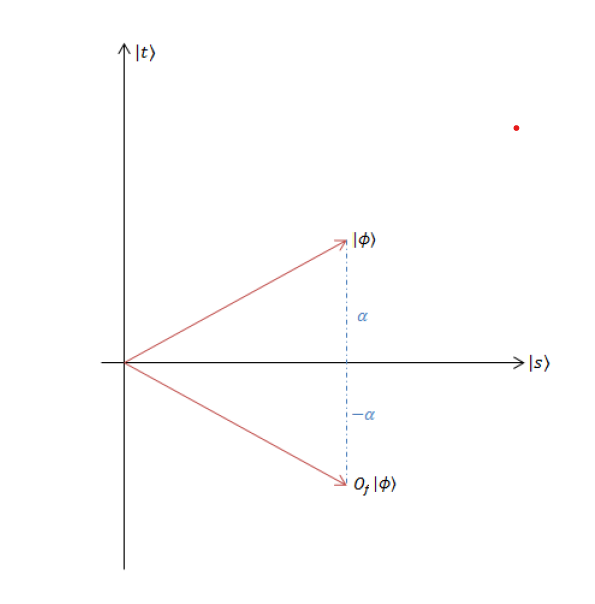
\includegraphics[width=10cm]{7_1.png}
	\label{fig:7-1}
\end{figure}
 
 بردارهای $\ket{v}$ و $\ket{w}$ را به صورت زیر تعریف کنید
 \begin{equation}
 \begin{split}
 & \ket{v} := \frac{1}{\sqrt{N}} \sum_{x \in \{0,1\}^{n}} \ket{x} \Rightarrow \ket{v} = \sqrt{\frac{N-1}{N}} \ket{s} + \frac{1}{\sqrt{N}} \ket{t} \\
 & \ket{w} :=  \frac{1}{\sqrt{N}} \ket{s} - \sqrt{\frac{N-1}{N}} \ket{t} \Rightarrow \braket{v}{w} = 0
 \end{split}
 \end{equation}
 تبدیل یکانی $U$ را در نظر بگیرید:
 \begin{equation}
 	U := H^{\otimes n}(2\dyad{0...0}{0...0} - I)H^{\otimes n} = 2H^{\otimes n}\dyad{0...0}{0...0}H^{\otimes n} - I
 \end{equation}
 می‌دانیم 
  \begin{equation}
  \begin{split}
  	& H^{\otimes n}\ket{0...0} = \frac{1}{\sqrt{2^{n}}} \sum_{x \in \{0,1\}^{n}} \ket{x} 
  	& = \frac{1}{\sqrt{N}} \sum_{x \in \{0,1\}^{n}} \ket{x} = \ket{v}
  \end{split}
  \end{equation}
  در نتیحه،
  \begin{equation}
  	U = 2\dyad{v}{v} - I
  \end{equation}
  و برای 
  $\ket{\psi} = \gamma\ket{v} + \lambda\ket{w}$ 
  داریم:
   \begin{equation}
   	U\ket{psi} = \gamma U \ket{v} + \lambda U \ket{w} = \gamma\ket{v} - \lambda\ket{w}
   \end{equation}
  نتیجه می‌شود که $U$ نسبت به $\ket{v}$ عمل قرینه انجام می‌دهد. (شکل \ref{fig:7-2})
\begin{figure}[h]
	\caption{ اعمال $U$ که در واقع عمل قرینه‌کردن نسبت به $\ket{v}$ است.}
	\centering
	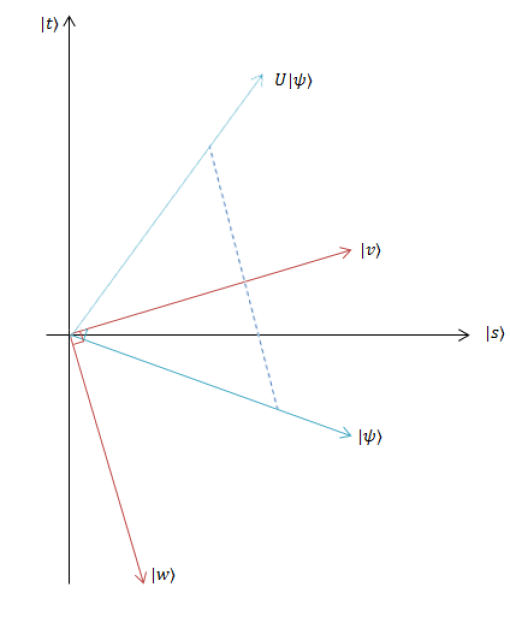
\includegraphics[width=10cm]{7_2.png}
	\label{fig:7-2}
\end{figure}

همانطور که می‌دانیم، ترکیب دو عمل قرینه، یک عمل دوران بدست می‌دهد. (شکل \ref{fig:7-3})
\begin{equation}
{f} = R_{2\theta}
\end{equation}
\begin{figure}[h]
	\caption{ $(2) = T_{f}(1), (3) = U(2)$}
	\centering
	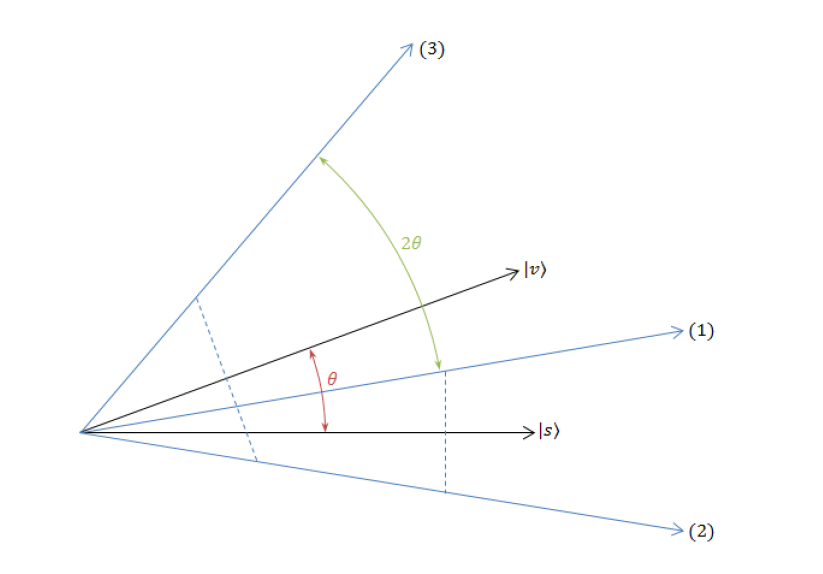
\includegraphics[width=10cm]{7_3.png}
	\label{fig:7-3}
\end{figure}
که در آن 
\begin{equation}
	cos \theta = \braket{v}{s} = \sqrt{\frac{N-1}{N}} \Rightarrow \theta \approx	\frac{1}{\sqrt{N}}
\end{equation}
\section{الگوریتم اصلی}
با $n$ کیوبیت که همگی در حالت $\ket{0}$ آماده‌سازی‌ شده‌اند شروع می‌کنیم. ابتدا، روی هر یک از $n$ کیوبیت عملگرد هامارد را اعمال می‌کنیم و بعد $R_{2 \theta}$ را $q$ بار و در آخر همه $n$ کیوبیت را اندازه‌گیری می‌کنیم: 
\begin{equation}
	\ket{0...0} \rightarrow^{H^{\otimes n}} \ket{v} \rightarrow^{(UT_{f})^{q}} \ket{\tau} \to measurement
\end{equation}
$\ket{\tau}$ یک بردار با زاویه $\theta + 2q\theta$ از $\ket{s}$ می‌باشد. اگر $q \approx \frac{\sqrt{N}}{4}\pi$ بگیریم، این زاویه تقریبا برابر با $\pi / 2$ خواهد بود. در این صورت  $\ket{\tau}$ تقریبا با $\ket{t}$ برابر است. حال با اندازه‌گیری $\tau$، حاصل اندازه‌گیری با احتمال 
\begin{equation}
	p(t) = \|\mel{t}{(UT_{f})^{q}}{v}\|^{2} = \|\braket{t}{\tau}
\end{equation}
برابر $t$ خواهد شد، و از آنجا که $\ket{t}$ و $\ket{\tau}$ به هم نزدیک است، این عدد نزدیک به $1$ است.